\begin{center}

  \begin{tabular}{rp{16cm}lp{20cm}}%{rl}

  % after \\: \hline or \cline{col1-col2} \cline{col3-col4} ...

  论文地址:& \href{https://arxiv.org/abs/1312.6114}{https://arxiv.org/abs/1312.6114} \\
  来源:& CoRR, 2013 \\
  作者:& Diederik P Kingma, Max Welling \\
  %源码:& \href{xxx}{xxx} \\

%  slides:& \href{http://yunshengb.com/wp-content/uploads/2017/03/nips_2018_r2l_workshop_talk.pdf}{{\footnotesize Convolutional Set Matching for Graph Similarity}}\\

  关键词:& \textbf{Variational Bayes, Auto-Encoding, Bayes Inference, Probalistic Model} \\

  写于:& \date{220-11-09}

  \end{tabular}

\end{center}

论文\cite{kingma2014autoencoding}为bayes概率图模型难以求解的问题提供了一种有效的思路,利用auto-encoding方法结合variational lower bound求解bayes图模型隐变量的后验分布。

在推断和学习中,我们可以认为数据是根据某个隐变量生成的 --- 可以从数据得到隐变量,也能够根据隐变量得到数据 --- 就像一个编码、解码的过程。但是,通常隐变量的分布是未知的、复杂的,难以通过假定一个已知的分布来近似隐变量的真实分布。

简单谈一下个人对隐变量的理解:宽泛的讲,隐变量就像现实背后的某种神秘的、未知的因素,我们所见的现实背后蕴含着这种神秘的因素 --- 隐变量,但我们通常是看不到隐变量的,也无法对它进行直接的观测,比如直接描述它是什么、它的形式、它发生的概率等等。但当我们得知隐变量后我们就像获得了某种神奇的力量,知道隐变量发生后现实中会发生什么。从数据的角度来看,隐变量可以是数据背后的“真理” --- 特征、数据产生的原因。当我们能够描述隐变量后,我们就能够根据隐变量生成我们想要的数据。这就像一个编码-解码的过程,将原始数据编码为特征,再根据特征产生数据。

\begin{figure}[h]
	\centering
	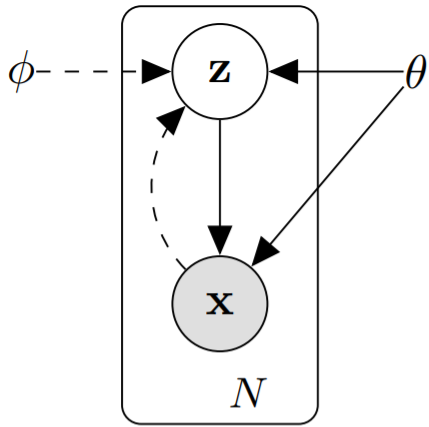
\includegraphics[width=.18\textwidth]{pics/AEVB.PNG}
	\caption{有向图模型}
	\label{fig:aevb}
\end{figure}

那么问题来了:\tbc{red}{如何得到隐变量呢?}

如图\ref{fig:aevb}所示,图中实线可以看作生成(即解码)过程 --- $p_{\theta}(\boldsymbol{z})p_{\theta}(\boldsymbol{x}|\boldsymbol{z})$,虚线可以看作编码过程 --- $q_{\phi}(\boldsymbol{z}|\boldsymbol{x})$。$\theta$表示真实的分布的参数,$\phi$表示近似ho后验分布的参数 --- 该近似分布用于近似真实的后验分布$p_{\theta}(\boldsymbol{z}|\boldsymbol{x})$。为了使近似分布$q_{\phi}(\boldsymbol{z}|\boldsymbol{x})$和真实分布$p_{\theta}(\boldsymbol{z}|\boldsymbol{x})$尽量相同,可以使用KL散度进行衡量。

\begin{equatiopn}%\nonumber
	\begin{align}
		KL(q_{\phi}(\boldsymbol{z}|\boldsymbol{x})||p_{\theta}(\boldsymbol{z}|\boldsymbol{x})) &= E_{q_{\phi}(\boldsymbol{z}|\boldsymbol{x})}[ \log \frac{q_{\phi}(\boldsymbol{z}|\boldsymbol{x})}{p_{\theta}(\boldsymbol{z}|\boldsymbol{x})} ] \notag \\
		&= E_{q_{\phi}(\boldsymbol{z}|\boldsymbol{x})}[ \log q_{\phi}(\boldsymbol{z}|\boldsymbol{x}) - \log {p_{\theta}(\boldsymbol{z}|\boldsymbol{x})} ] \notag \\
		&= E_{q_{\phi}(\boldsymbol{z}|\boldsymbol{x})}[ \log q_{\phi}(\boldsymbol{z}|\boldsymbol{x}) - \log \frac{p_{\theta}(\boldsymbol{z},\boldsymbol{x})} {p_{\theta}(\boldsymbol{x})} ] \notag \\
		&= E_{q_{\phi}(\boldsymbol{z}|\boldsymbol{x})}[ \log q_{\phi}(\boldsymbol{z}|\boldsymbol{x}) - \log p_{\theta}(\boldsymbol{z},\boldsymbol{x}) + \log p_{\theta}(\boldsymbol{x}) ] \notag \\
		&= E_{q_{\phi}(\boldsymbol{z}|\boldsymbol{x})}[ \log q_{\phi}(\boldsymbol{z}|\boldsymbol{x}) - \log p_{\theta}(\boldsymbol{z},\boldsymbol{x})] + \log p_{\theta}(\boldsymbol{x})   \label{eq:kl}
	\end{align}
\end{equatiopn}
由公式(\ref{eq:kl})可得,对于训练数据中的每一个样本有:
$$
\log p_{\theta}(\boldsymbol{x}^{(i)}) = KL(q_{\phi}(\boldsymbol{z}|\boldsymbol{x}^{(i)})||p_{\theta}(\boldsymbol{z}|\boldsymbol{x}^{(i)})) + \mathcal{L}(\theta, \phi; \boldsymbol{x}^{(i)})
$$
其中,
$$\mathcal{L}(\theta, \phi; \boldsymbol{x}^{(i)}) = E_{q_{\phi}(\boldsymbol{z}|\boldsymbol{x})}[ -\log q_{\phi}(\boldsymbol{z}|\boldsymbol{x}) + \log p_{\theta}(\boldsymbol{z},\boldsymbol{x})]
$$
因为KL是大于等于零的,那么显然有这样的关系:$\log p_{\theta}(\boldsymbol{x}^{(i)}) \ge \mathcal{L}(\theta, \phi; \boldsymbol{x}^{(i)})$。所以$\mathcal{L}(\theta, \phi; \boldsymbol{x}^{(i)})$又叫做变分下界(variational lower bound)。$\log p_{\theta}(\boldsymbol{x}^{(i)})$相当于样本的对数似然函数,当给定了数据后,其实$\log p_{\theta}(\boldsymbol{x}^{(i)})$应该是确定的,那么为了使近似分布尽量接近真实分布,那么则应该让变分下界尽可能的大,这样近似分布就会尽可能地接近真实分布。OKAY!现在问题转化成了最大化$\mathcal{L}(\theta, \phi; \boldsymbol{x}^{(i)})$了。

那么问题又来了:\tbc{red}{如何最大化变分下界呢?}

经过一顿操作后,变分下界可写为:
$$\mathcal{L}(\theta, \phi; \boldsymbol{x}^{(i)}) = -KL(q_{\phi}(\boldsymbol{z}|\boldsymbol{x}^{(i)})||p_{\theta}(\boldsymbol{z})) + E_{q_{\phi}(\boldsymbol{z}|\boldsymbol{x}^{(i)})}[\log p_{\theta}(\boldsymbol{x}^{(i)}|\boldsymbol{z})]
$$
其中第一项可以看作正则化项(当增加隐变量的数量时,可以防止过拟合),第二项可以看作重构损失。为了最大化变分下界,可以使用梯度下降的方法,但是上式中变分下界难以计算,且近似分布$q_{\phi}(\boldsymbol{z}|\boldsymbol{x}^{(i)})$是未知的。如果直接使用蒙特卡洛方法计算变分下界,将会带来较大方差。论文中针对这个问题使用了重参数化(reparameterization)来表示隐变量:$\hat{\boldsymbol{z}} = g_{\phi}(\boldsymbol{\epsilon}, \boldsymbol{x})$,其中$\boldsymbol{\epsilon}$服从于某个分布$p(\boldsymbol{\epsilon})$。那么问题就转化成了选择合适的函数$g$和分布$p(\boldsymbol{\epsilon})$。已知一个函数关于其自变量的后验分布的的蒙特卡洛估计为下式:
$$
E_{q_{\phi}(\boldsymbol{z}|\boldsymbol{x}^{(i)})}[f(\boldsymbol{z})] = E_{p(\boldsymbol{\epsilon})}[f(g_{\phi}(\boldsymbol{\epsilon}, \boldsymbol{x}^{(i)} ) ) ] \simeq \frac{1}{L} \sum_{l=1}^{L} f(g_{\phi}(\boldsymbol{\epsilon}^{(l)}, \boldsymbol{x}^{(i)} ) )
$$
其中$L$为对每个数据$\boldsymbol{x}^{(i)}$进行蒙特卡洛采样的次数。那么使用蒙特卡洛估计重参数化后的变分下界,形式为:
$$
\mathcal{L}(\theta, \phi; \boldsymbol{x}^{(i)}) =  \frac{1}{L} \sum_{l=1}^{L} \log p_{\theta}(\boldsymbol{z}^{(i, l)},\boldsymbol{x}^{(i)}) - \log q_{\phi}(\boldsymbol{z}^{(i, l)}|\boldsymbol{x}^{(i)})
$$
其中,$\boldsymbol{z}^{(i, l)}=g_{\phi}(\boldsymbol{\epsilon}{(i, l)}, \boldsymbol{x}{(i)}), \boldsymbol{\epsilon}^{(l)} \sim p(\boldsymbol{\epsilon})$。之后便可以使用小批量的随机梯度下降算法优化参数$\theta, \phi$。

关于VAE的tutorial可以参考:\href{https://arxiv.org/pdf/1606.05908.pdf}{Tutorial on Variational Autoencoders}。未使用重参数化技巧与使用了重参数化技巧对比如Fig.\ref{fig:vae_rp}\cite{doersch2016tutorial}所示:
\begin{figure}[h]
	\centering
	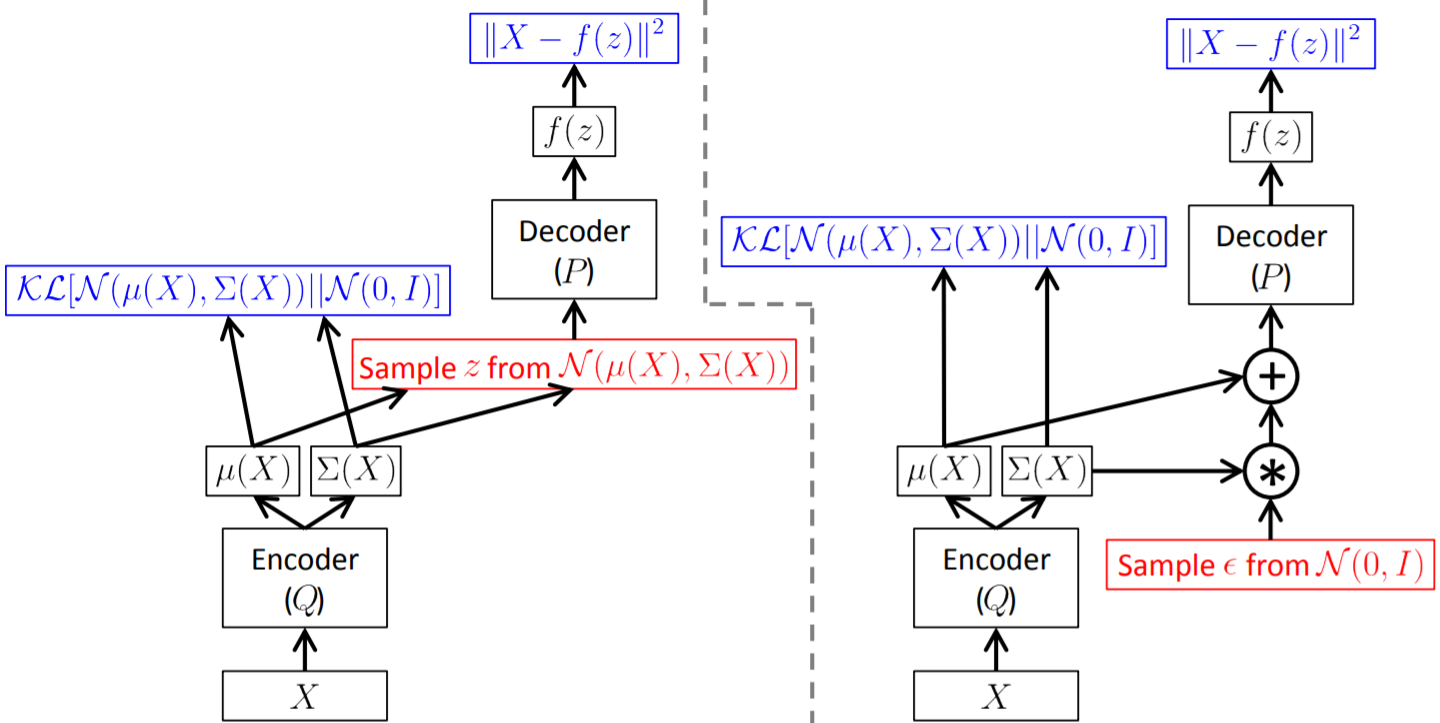
\includegraphics[width=.8\textwidth]{pics/vae_rp.png}
	\caption{without vs. with reparameterization}
	\label{fig:vae_rp}
\end{figure}

一些网上的参考资料:
\begin{itemize}
	\item \href{https://www.cnblogs.com/yifdu25/p/8181185.html}{变分推断}
\end{itemize}

\paragraph{方法解决的问题/优势}

\begin{itemize}
	\item 从参数化变分下界,使得能够使用随机梯度下降算法优化参数
	%\item 

\end{itemize}


\paragraph{方法的局限性/未来方向}

\begin{itemize}
	\item 时序模型
	\item 具有隐变量的监督学习模型,可用于学习复杂的噪声分布

\end{itemize}






